\hypertarget{NeutronPrimaryGeneratorAction_8cc}{}\section{src/\+Neutron\+Primary\+Generator\+Action.cc File Reference}
\label{NeutronPrimaryGeneratorAction_8cc}\index{src/\+Neutron\+Primary\+Generator\+Action.\+cc@{src/\+Neutron\+Primary\+Generator\+Action.\+cc}}


constructs the particle gun and initializes the particle generation when used as a user action in the \hyperlink{classNeutronActionInitialization}{Neutron\+Action\+Initialization} class  


{\ttfamily \#include \char`\"{}Neutron\+Primary\+Generator\+Action.\+hh\char`\"{}}\newline
{\ttfamily \#include \char`\"{}G\+T\+K\+Input.\+hh\char`\"{}}\newline
{\ttfamily \#include \char`\"{}G4\+System\+Of\+Units.\+hh\char`\"{}}\newline
{\ttfamily \#include \char`\"{}G4\+Particle\+Definition.\+hh\char`\"{}}\newline
{\ttfamily \#include \char`\"{}G4\+Particle\+Gun.\+hh\char`\"{}}\newline
{\ttfamily \#include \char`\"{}G4\+Particle\+Table.\+hh\char`\"{}}\newline
{\ttfamily \#include \char`\"{}Randomize.\+hh\char`\"{}}\newline
Include dependency graph for Neutron\+Primary\+Generator\+Action.\+cc\+:
\nopagebreak
\begin{figure}[H]
\begin{center}
\leavevmode
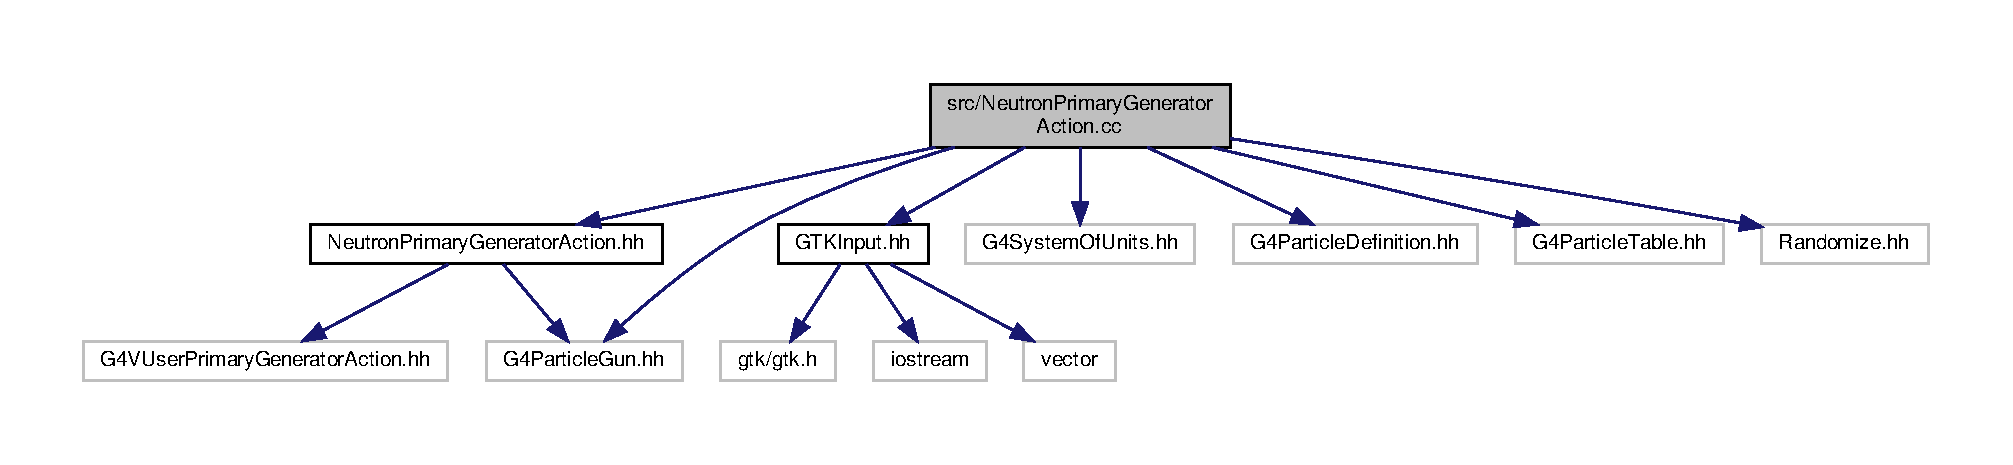
\includegraphics[width=350pt]{NeutronPrimaryGeneratorAction_8cc__incl}
\end{center}
\end{figure}


\subsection{Detailed Description}
constructs the particle gun and initializes the particle generation when used as a user action in the \hyperlink{classNeutronActionInitialization}{Neutron\+Action\+Initialization} class 

\begin{DoxyAuthor}{Author}
Oisin O\textquotesingle{}Connell
\end{DoxyAuthor}
\begin{DoxyDate}{Date}
7/20/20 
\end{DoxyDate}
